\documentclass[a4paper,dvipsnames]{article}

\input ../header
\newcommand{\checkedbox}{\makebox[0pt][l]{$\square$}\raisebox{.15ex}{\hspace{0.1em}$\checkmark$}}
\newcommand{\checkbox}{\makebox[0pt][l]{$\square$}\raisebox{.15ex}{\hspace{0.1em}}\hspace{3mm}}

\begin{document}

\title{Évaluation 6 -- Sujet A}
\author{}
\date{}

\maketitle{}

\pagestyle{empty}
\thispagestyle{empty}

% Exercice sur les fractions
\exo[3 points] Effectuer les calculs suivants. Donner le résultat sous la forme d'une fraction irréductible.
\begin{multicols}{4}
  \begin{enumerate}
    \item $\dfrac{3}{4} + \dfrac{4}{5}\vphantom{\dfrac{\dfrac{1}{2}}{\dfrac{3}{4}}}$\columnbreak
    \item $\dfrac{7}{6} - \dfrac{5}{4}\vphantom{\dfrac{\dfrac{1}{2}}{\dfrac{3}{4}}}$\columnbreak
    \item $\dfrac{9}{20} \times \dfrac{25}{4}\vphantom{\dfrac{\dfrac{1}{2}}{\dfrac{3}{4}}}$\columnbreak
    \item $\cfrac{\phantom{1}\dfrac{12}{5}\phantom{1}}{\dfrac{18}{25}}$
  \end{enumerate}
\end{multicols}
\dotfill\rep{16}

\bigskip

% Exercices sur les quotients
\exo[3 points] Réduire au même dénominateur afin d'écrire les expressions suivantes sous la forme d'un unique quotient.
\begin{multicols}{2}
  \begin{enumerate}
    \item $5-\dfrac{2}{3x-2}$
    \item $\dfrac{3x}{2x-1}+\dfrac{4x+9}{x}$
  \end{enumerate}
\end{multicols}
\dotfill\rep{22}

\pagebreak

% Exercice de probabilités
\exo[3 points]\vspace*{-6mm}

\begin{multicols}{2}
  La roue représentée ci-contre est divisée en cinq secteurs. On réalise l'expérience aléatoire suivante : on fait tourner la roue et on note la lettre du secteur coloré sur lequel la roue s'immobilise.

  \begin{enumerate}
    \item Modéliser cette expérience aléatoire.\rep{6}
      \begin{center}
	\vspace*{1mm}\hspace*{7mm}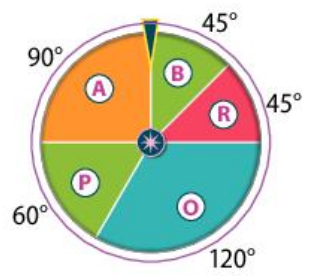
\includegraphics[width=5cm]{evaluation_6_roue.png}
      \end{center}
  \end{enumerate}
\end{multicols}

\begin{enumerate}
  \setcounter{enumi}{1}
  \item Déterminer la probabilité des événements suivants :
  \begin{enumerate}
    \item \og{}on obtient une voyelle\fg{} ;\rep{5}
    \item \og{}on obtient une lettre du mot \textsc{FOOTBALL}\fg{} ;\rep{5}
    \item \og{}on obtient une lettre appartenant à un secteur vert\fg{}.\rep{5}
  \end{enumerate}
\end{enumerate}

\bigskip

% Exercice sur les fonctions
\exo[3 points] Josh, qui s'est installé à Moorea, loue des vélos. Il propose un forfait de $\np{3000}$ XPF pour $4$ heures de location. Au-delà, chaque heure supplémentaire est facturée $500$ XPF.
\begin{enumerate}
  \item Aaron loue un vélo et l'utilise pendant $3$ heures. Combien paiera-t-il la location ?\rep{5}
  \item Mihiau loue un vélo pendant $6$ heures. Combien paiera-t-elle la location ?\rep{5}
  \item Compléter le code ci-dessous afin que la fonction \mintinline{python}{cout} prenne en paramètre la durée de location (en heures) et renvoie le coût de celle-ci :
    \begin{minted}{python}
def cout(...):
    if .........:
        C = .........
    else:
        C = .........
    return ...
    \end{minted}
  \item Comment utiliser cette fonction pour connaître le coût de $7$ heures de location ?\rep{4}
\end{enumerate}

\end{document}
